% !TEX root = /home/computer/ucsc/master-2/quarter-2/advanced-fluids/master.tex
\assignment{2}{Sat 15 Jan 2022 20:20}{Assignment 2}

\subsectionfont{\fontsize{10}{10}\selectfont}

\graphicspath{./assignment_02/figures/}

\section{Sound waves with gravity}%

\textbf{Question 1}: Find the equation for isothermal sound waves in an
isothermal atmosphere without neglecting gravity.

Conservation of momentum including gravity (\ref{eq:1}), and conservation of mass
(\ref{eq:2})
\begin{gather} 
  \rho   \frac{D\bf{u}}{Dt} = -\nabla p + \rho\bf{g} \label{eq:1} \\
  \diffp[]{\rho}{t} + \nabla\cdot (\rho {\bf u}) = 0 \label{eq:2}
\end{gather}

Then considering small perturbations in a motionless and homogeneous background
state

\[
\begin{cases}
  p = p_0+\tilde{p} \\
  \rho = \rho_0 +   \tilde{\rho} \\
  \bf{u} = \underbrace{\bf{u}_{0}}_{=0} + \tilde{\bf{u}} = \tilde{\bf{u}}
\end{cases}
.\] 

Plugging these perturbations into the governing equations, expanding the
substantial derivative

\begin{gather*}
  (\rho_0 + \tilde{ \rho})\diffp[]{\bf{u}}{t} + (\rho_0+\tilde{\rho })\bf{u}
  \cdot \nabla \bf{u} = - \nabla (p_0+\tilde{p})+ (\rho_0+\tilde{\rho})\bf{g}
   \\
  \diffp[]{ (\rho_0+\tilde{\rho })}{t} + \nabla \cdot
  ((\rho_0+\tilde{\rho}){\bf u}) = 0
\end{gather*}

Ignoring quadratic terms in small perturbations, and using $\nabla p_0 =0$ and
$\nabla \rho_0 = 0$ for change in homogeneous steady state

\begin{gather}
  \rho_0 \diffp[]{\bf{\tilde{u}}}{t} = -\nabla \tilde{p}
  + (\rho_0+\tilde{\rho})\bf{g} \label{eq:3}\\
\diffp[]{\tilde{\rho }}{t} + \nabla \cdot (\rho_0{\bf u}) = 0 \label{eq:4}
\end{gather}

Taking the time derivative of $(\ref{eq:4})$ 
\begin{gather*}
\diffp[2]{\tilde{\rho }}{t} + \nabla \cdot \left( \rho_0 \diffp[]{{\bf
\tilde{u}}}{t}\right) = 0 \\
\end{gather*}

Plugging in RHS of $(\ref{eq:3})$ for $\rho_0 \diffp[]{{\bf \tilde{u}}}{t}$ 

\begin{gather*}
  \diffp[2]{\tilde{\rho }}{t} + \nabla \cdot \left(-\nabla \tilde{p}
  + (\rho_0+\tilde{\rho})\bf{g} \right) = 0 \\
  \diffp[2]{\tilde{\rho }}{t} = \nabla^{2}\tilde{p} - (\nabla \cdot \tilde{\rho
  }{\bf g}
  )
\end{gather*}

Considering ${\bf g} = \begin{pmatrix} 0 \\ 0 \\ -g \end{pmatrix}$
\begin{equation}
  \diffp[2]{\tilde{\rho }}{t} = \nabla ^{2}\tilde{p} + g \diffp[]{\tilde{\rho
  }}{z} \label{eq:5}
\end{equation}

Linearizing around the EOS for an isothermal, $T = T_0$, perfect gas $p
= R \rho T_0$, and assuming temperature pertubations diffuse rapidly,
$\tilde{T} = 0$, we get the following relationship between $\tilde{p}$ and
$\tilde{\rho }$ 

\begin{equation}
  \tilde{p} = RT_0\tilde{\rho } \label{eq:6}
\end{equation}

Letting $c^{2}=RT_0$, and plugging this, $(\ref{eq:6})$, into $(\ref{eq:5})$ 
\begin{equation}
  \boxed{\diffp[2]{\tilde{\rho }}{t} = c^{2}\nabla ^{2}\tilde{\rho
  } + g \diffp[]{\tilde{\rho }}{z}} \label{eq:7}
\end{equation}

\textbf{Question 2}: Ignoring $x$ and $y$ components, and plugging in the
 monochramatic wave solution $\rho (z,t) = \hat{\rho
} e^{ikz-i \omega t}$ in to $(\ref{eq:7})$ with
\begin{gather*}
  \diffp[]{\rho }{z} = ik \rho  , \quad
  \diffp[2]{\rho }{z} = -k^{2}\rho \\
  \diffp[2]{\rho }{t} = -\omega ^{2}\rho \\
\end{gather*}

and simplifying, we get the dispersion relation
\begin{gather}
  -\omega ^{2}\rho = -c^{2}k^{2}\rho + ik\rho g \nonumber \\
  \boxed{\omega^{2} = c^2 k^2 \left(1-i \frac{g}{kc^2}\right)} \label{eq:8}
\end{gather}


The term that includes gravity is negligible when 
\[
kc^2\gg g
.\] 

using $g = 9.8\frac{m}{s^2}$, $c=290
\frac{m}{s}$, and frequency $\omega = 3000$ Hz, we can see that $\frac{g}{c^2}
= 0.000116527942925089$. If we assume that this is already negligible then $k=
\frac{\omega}{c} = 10.3448275862069$. This is of course already assuming that
gravity is negligible, but seems unlikely to be off by a factor of $10$.
A similar analysis suggests that gravity may not be negligible for very low
frequency.

\section{Superposition of monochromatic waves vs. d'Alembert's solution}%
\label{sec:2}

Solve the $1$D Cartesian wave equation on domain $t>0$, and $-\infty<x<\infty$
\begin{gather*}
    p_{tt} = c^2p_{xx} \\
    p(x,0) = f(x) \\
    p_{t}(x,0) = g(x)
\end{gather*}

Applying the Fourier transform in $x$, then Fourier coefficient $\hat{p}_{xx}=
(ik)^2\hat{p}$, and
\[
  \hat{p}_{tt}(k,t) = - (ck)^2\hat{p}(k,t)
.\] 

Which is an ODE in time with solution
\begin{equation}
  \hat{p}(k,t) = Ae^{ickt}+Be^{-ickt} \label{eq:9}
\end{equation}

with initial conditions
\begin{align*}
  \hat{p}(k,0) &= \frac{1}{\sqrt{2\pi}} \int_{-\infty }^{\infty
  } { \underbrace{p(x,0)}_{=f(x)}e^{-ikx}} \: d{x} \\
  &= \hat{f}(k) \qquad \text{and, }\\
  \hat{p}_{t}(k,0) &= \hat{g}(k)
\end{align*}

Applying these to the general solution (\ref{eq:9}), we get
  \begin{gather*}
    A = \frac{1}{2} \left(\hat{f}+ \frac{\hat{g}}{ick}\right) \\
    B = \frac{1}{2} \left(\hat{f}- \frac{\hat{g}}{ick}\right) \\
  \end{gather*}

then the solution is
\[
  \hat{p}(k,t) = \frac{1}{2} \left(\hat{f}+ \frac{\hat{g}}{ick}\right)e^{ickt}
  + \frac{1}{2} \left(\hat{f}- \frac{\hat{g}}{ick}\right)e^{-ickt}
.\] 

Applying the inverse Fourier transform
\begin{align*}
    p(x,t) &= \frac{1}{\sqrt{2\pi }} \int_{-\infty }^{\infty
  } {\frac{1}{2}\hat{f}(k)e^{ik (x+ct)} + \frac{1}{2}\hat{f}(k)e^{ik (x-ct)}}
  \: d{k} \\
  &+ \frac{1}{\sqrt{2\pi }} \int_{-\infty }^{\infty
  } {\frac{1}{2ick}\hat{g}(k)e^{ik (x+ct)} - \frac{1}{2ick}\hat{g}(k)e^{ik (x-ct)}}
  \: d{k}
\end{align*}

we recover d Alembert's solution first noting that
\[
  f(x \pm ct) = \frac{1}{\sqrt{2\pi }} \int_{-\infty }^{\infty
  } {\hat{f}(k)e^{ik (x\pm ct)}} \: d{k} 
.\] 

and
\begin{align*}
  &\frac{1}{\sqrt{2\pi }} \int_{-\infty }^{\infty
  } {\frac{1}{2ick}\hat{g}(k)e^{ik (x+ct)} - \frac{1}{2ick}\hat{g}(k)e^{ik (x-ct)}}
  \: d{k} \\
  & \quad = \frac{1}{\sqrt{2\pi }} \int_{-\infty }^{\infty}
  {\frac{1}{2cik}\hat{g}(k) e^{ik\xi}\biggr|_{x-ct}^{x+ct}} \: d{k} \\
  & \quad = \frac{1}{\sqrt{2\pi }} \int_{-\infty }^{\infty
  } {\frac{1}{2c}\hat{g}(k) \int_{x-ct}^{x+ct} {e^{ik\xi}} \: d{\xi} 
  } \: d{k} \\
  & \quad = \frac{1}{2c} \int_{x-ct}^{x+ct} {g(\xi)} \: d{\xi} 
\end{align*}

putting everything together
\[
  p(x,t) = \frac{1}{2} \left(f(x-ct) + f(x+ct)\right) + \frac{1}{2c} \int_{x-ct}^{x+ct} {g(\xi)} \: d{\xi} 
.\] 

if $p_{t}(x,0) = g(x) = 0$, and $f(x) = p_0 e^{-\frac{x^2}{2}}$ then
\[
  \boxed{p(x,t) = \frac{1}{2}p_0 \left(e^{-\frac{(x-ct)^2}{2}} + e^{-\frac{(x+ct)^2}{2}}\right)}
.\] 

\section{Global modes in a square}%
\label{sec:3}

Find the $2$D eigenmodes and eigenvalues of the wave equation in a square with
side length $1$ 
  \[
  \diffp[2]{p}{t} = c^2\nabla ^2p
  .\] 
subject to $p=0$ on the boundary
\begin{align*}
  p(0,y,t) = p(1,y,t) = 0 \qquad y\in [0,1] \\
  p(x,0,t) = p(x,1,t) = 0 \qquad x\in [0,1]
\end{align*}

Using separation of variables for a solution of the form
\[
  p(x,y,t) = X(x)Y(y)T(t)
.\] 
and plugging this into the wave equations
\begin{gather*}
  XYT^{\prime\prime} = c^2 \left(X^{\prime\prime}YT
  + XY^{\prime\prime}T\right) \\
  \frac{T''}{c^2T} = \frac{X''}{X} + \frac{Y''}{Y}
\end{gather*}

Since both sides are functions of different variables, in order for them to
equate, they must be equal to a constant
\[
  \frac{T''}{c^2T} = \frac{X''}{X} + \frac{Y''}{Y} = A
.\] 

So we have
\begin{gather}
  T'' = c^2AT \nonumber \\
  \frac{X''}{X} = A - \frac{Y''}{Y} = B \label{eq:10}
\end{gather}

where (\ref{eq:10}) must equal another constant. Defining $C = A-B$, we get
\begin{gather*}
  X'' = BX \\
  Y'' = CY
\end{gather*}

Considering the different cases for sign of $B$ and  $C$, only $B < 0$ and $C
<0$ lead to non trivial solutions. Applying boundary conditions and
ignoring the constant in front of solutions
\[
\begin{cases}
  X_{ \omega }(x) = \sin (\omega \pi x), &\text{ for } \omega = 1,2,3,\dots \\
  Y_{k}(y) = \sin (k\pi y), &\text{ for } k = 1,2,3,\dots \\
\end{cases}
.\] 

where $B = - (\omega \pi)^2$ and $C = - (k \pi )^2$ implies $ A = - ( (\omega
\pi )^2 + (k \pi )^2)$. Defining $ \lambda_{\omega ,k} = c^2A $, then
\[
  \lambda _{(\omega ,k)}^2 = - ( (c \omega \pi )^2 + (c k \pi )^2) < 0
.\] 

and $T(t)$ has solution
\[
  T_{(\omega ,k)}(t) = a\cos \left( \lambda _{(\omega ,k)}t \right) + b\sin
  \left(  \lambda _{(\omega ,k)} t\right)
.\] 

So the eigenmodes (\ref{eq:11})
\begin{gather}
  p_{\omega, k}(x,y,t) = X_{ \omega }(x)Y_{ k}(y)T_{ \omega,k }(t) \nonumber \\
   \boxed{p_{\omega, k}(x,y,t) = \sin (\omega \pi x)\sin (k \pi y) \left( a\cos
   \left( \lambda _{(\omega ,k)}t \right) + b\sin \left(  \lambda _{(\omega
   ,k)} t\right)\right)} \label{eq:11}
\end{gather}

and eigenvalues (\ref{eq:12})
\begin{gather}
  \boxed{\lambda _{ (\omega ,k)} = c \pi \sqrt{ \omega ^2 + k^2}} \label{eq:12}
\end{gather}

where coefficients $a$ and $b$ are found using initial conditions. Letting $a
= b = 1$, and plotting different modes

\begin{figure}[H]
  \centering
  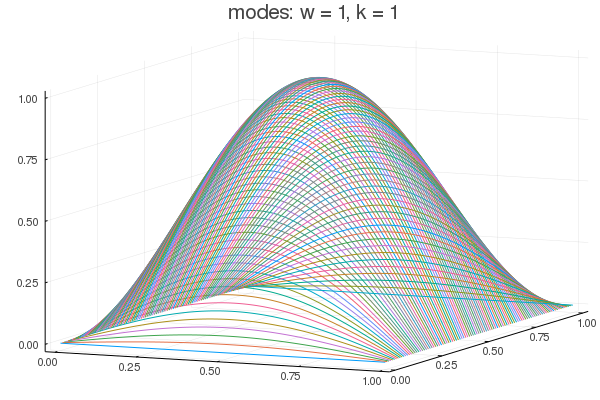
\includegraphics[width=0.8\linewidth]{./assignment_02/figures/modes_w1_k1.png}
  \caption{modesw1k1}%
  \label{fig:modesw1k1}
\end{figure}
\begin{figure}[H]
  \centering
  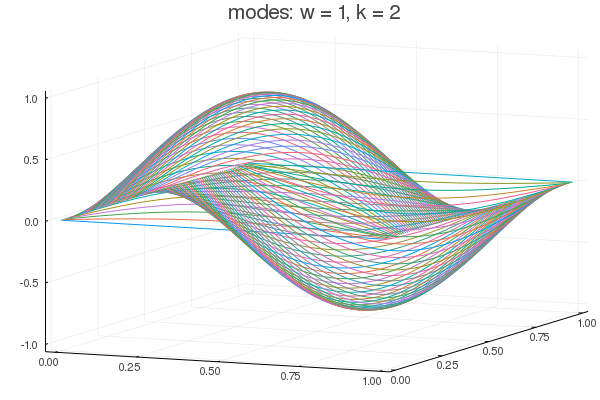
\includegraphics[width=0.8\linewidth]{./assignment_02/figures/modes_w1_k2.png}
  \caption{modesw1k2}%
  \label{fig:modesw1k2}
\end{figure}
\begin{figure}[H]
  \centering
  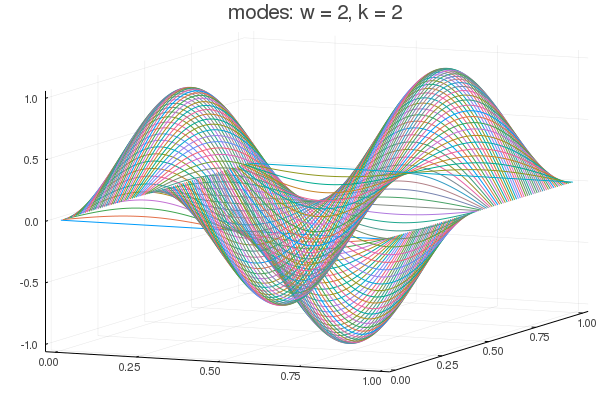
\includegraphics[width=0.8\linewidth]{./assignment_02/figures/modes_w2_k2.png}
  \caption{modesw2k2}%
  \label{fig:modesw2k2}
\end{figure}

\section{Multi scale expansion for the damped oscillator}%
\label{sec:4}

\textbf{Actual Question}: Consider the ODE
\begin{gather*}
  \diff[2]{f}{t}+f= -\epsilon \diff[]{f}{t} \\
  f(0) = 1 \\
  \diff[]{f(0)}{t} = 0
\end{gather*}

Write $f(t) = f(T_{s}(t),T_{f}(t))$ where $T_{s}=\epsilon t$ is the slow time and
$T_{f} = t$ is the fast time. Using the chain rule 

\begin{align*}
  \diff[]{f}{t} &= \diffp[]{f}{T_{s}}\diff[]{T_{s}}{t} + \diffp[]{f}{T_{f}}
  \diff[]{T_{f}}{t} \\
                &= \epsilon \diffp[]{f}{T_{s}} + \diffp[]{f}{T_{f}} \\
                &= \epsilon \diffp[]{f}{T_{s}} + \diffp[]{f}{t}
\end{align*}

Letting $T = T_{s}$, and assuming solution is of the form $f(T,t) = A(T)e^{i
\theta(t)}$ where amplitude is a slowly varying function of time and frequency
is a fast varying function of time. Then, using $ \omega = - \diffp[]{\theta}{t}$
\begin{align*}
  \diff[]{f}{t} &= \epsilon \diff[]{A}{T}e^{i\theta } + i \diff[]{\theta
  }{t}Ae^{i \theta } \\
  &= \epsilon \diff[]{A}{T} - i \omega f
\end{align*}

and
\begin{align*}
  \diffp[2]{f}{t} &= \left(\epsilon \frac{\partial}{\partial T}
  + \frac{\partial}{\partial t}\right) \left(\epsilon \diffp[]{f}{T}
+ \diffp[]{f}{t} \right) \\
                  &= \left(\epsilon \frac{\partial}{\partial T}
  + \frac{\partial}{\partial t}\right) \left(\epsilon \diff[]{A}{t}e^{i\theta
  } + Ai \diff[]{\theta }{t}e^{i \theta }\right) \\
  &= -\omega ^2 A e^{i \theta } - 2i\epsilon \omega \diff[]{A}{T}e^{i \theta
  } - i \epsilon \diff[]{\omega}{T} A e^{i \theta } + O (\epsilon ^2)
\end{align*}

equating constant terms in resulting ODE
\begin{align*}
  -&\omega ^2 f + f = 0 \\
  &\implies (-\omega^2+1)f = 0\\
  &\implies \omega = \pm 1 \\
  &\implies \diff[]{\theta }{t} = \pm 1 \\
\end{align*}
\[
  \boxed{\implies \theta(t) = \pm t + c_{1,2}}
.\] 

equating $O (\epsilon )$ terms
\begin{gather*}
  -2i \epsilon \omega \diff[]{A}{T}e^{i \theta } - \underbrace{i \epsilon
  \diff[]{\omega }{T}f}_{=0} = i \omega \epsilon f \\
  \diff[]{A}{T} = -\frac{1}{2}A \\
  \boxed{\implies A(T) = A_0e^{-\frac{T}{2}}}
\end{gather*}

Finally the general solution is

\[
  \boxed{f(t) = e^{-\frac{\epsilon}{2}t} \left(c_1e^{it} + c_2e^{-it}\right)}
.\] 

which is exactly what you'd get solving the equation $f_{tt}+\epsilon f_{t}+f
=0$ directly using the anzatz $f(t) = e^{rt}$ or any other second order method.
